% !TEX root = ../Report.tex

Since hardware specifications and computational power increased dramatically in the last years machine learning approaches can be applied in various disciplines today. On top of that the progress in research on convolutional neuronal networks (CNN) made it a very powerful tool for image processing where information is gained from image data.\newline
One challenging application is medical image computing (MIC). The main goal of MIC is to extract clinically relevant information or knowledge from medical images. Furthermore Segmentation is the process of partitioning an image into different meaningful segments (e. g. organs, bones, ...).\newline
In this project the goal is to segment the lung of a human body from a computed tomography (CT) scans.\newline
The used dataset is from the LUNA16 challenge \cite{luna} and each scan contains a number of slices which are 512 x 512 pixel greyscale images. The algorithm creates a 512 x 512 pixel label map for each slice marking every pixel that is part of the lung. An example of one scan and the corresponding labeling is shown in figure \ref{scan_picture}.

\begin{figure}[h!]
	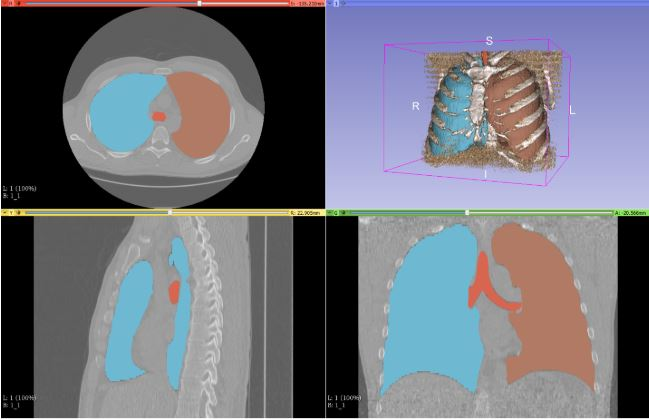
\includegraphics[width=0.49\textwidth, angle=0]{files/scan_picture.jpg}
	\caption{CT scan of the lung and labeled parts}
	\label{scan_picture}
\end{figure}

The segmentation of the lung from the rest of the picture is the first step for further image processing. In the LUNA16 dataset the final goal for example is to detect nodules of the lung indicating cancer. Machine learning approaches can be a powerful support for the doctors who treat patients with suspected cancer. The algorithms can reduce human errors and . It might even have the potential to outperform human capabilities and could automatizes the process of cancer detection. This could have a positive effect on health care quality and costs.\newline
In this work two different neuronal networks will be trained and tested to segment the lung on the above described dataset. Furthermore they will be examined and compared under different metrics.
First the DeepMedic Network and the UNet will be explained and related to other approaches for medical image segmentation. 
... 
